% AUTO-GENERATED by code/figlib.py helpers -- do not edit
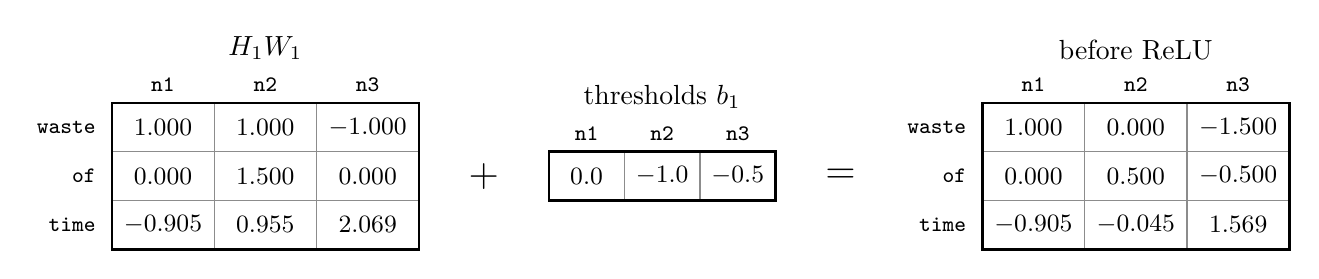
\begin{tikzpicture}
\draw[black!45, fill=white] (0.975,0.930) rectangle (2.275,0.310);
\node[font=\small, text=black] at (1.625,0.620) {$1.000$};
\draw[black!45, fill=white] (2.275,0.930) rectangle (3.575,0.310);
\node[font=\small, text=black] at (2.925,0.620) {$1.000$};
\draw[black!45, fill=white] (3.575,0.930) rectangle (4.875,0.310);
\node[font=\small, text=black] at (4.225,0.620) {$-1.000$};
\draw[black!45, fill=white] (0.975,0.310) rectangle (2.275,-0.310);
\node[font=\small, text=black] at (1.625,-0.000) {$0.000$};
\draw[black!45, fill=white] (2.275,0.310) rectangle (3.575,-0.310);
\node[font=\small, text=black] at (2.925,-0.000) {$1.500$};
\draw[black!45, fill=white] (3.575,0.310) rectangle (4.875,-0.310);
\node[font=\small, text=black] at (4.225,-0.000) {$0.000$};
\draw[black!45, fill=white] (0.975,-0.310) rectangle (2.275,-0.930);
\node[font=\small, text=black] at (1.625,-0.620) {$-0.905$};
\draw[black!45, fill=white] (2.275,-0.310) rectangle (3.575,-0.930);
\node[font=\small, text=black] at (2.925,-0.620) {$0.955$};
\draw[black!45, fill=white] (3.575,-0.310) rectangle (4.875,-0.930);
\node[font=\small, text=black] at (4.225,-0.620) {$2.069$};
\draw[line width=0.9pt] (0.975,0.930) rectangle (4.875,-0.930);
\node[anchor=east, font=\footnotesize\ttfamily] at (0.895,0.620) {waste};
\node[anchor=east, font=\footnotesize\ttfamily] at (0.895,-0.000) {of};
\node[anchor=east, font=\footnotesize\ttfamily] at (0.895,-0.620) {time};
\node[anchor=south, font=\footnotesize\ttfamily] at (1.625,0.950) {n1};
\node[anchor=south, font=\footnotesize\ttfamily] at (2.925,0.950) {n2};
\node[anchor=south, font=\footnotesize\ttfamily] at (4.225,0.950) {n3};
\node[anchor=south, font=\normalsize] at (2.925,1.350) {$H_1W_1$};
\node[font=\Large] at (5.700,0) {$+$};
\draw[black!45, fill=white] (6.525,0.310) rectangle (7.485,-0.310);
\node[font=\small, text=black] at (7.005,0.000) {$0.0$};
\draw[black!45, fill=white] (7.485,0.310) rectangle (8.445,-0.310);
\node[font=\small, text=black] at (7.965,0.000) {$-1.0$};
\draw[black!45, fill=white] (8.445,0.310) rectangle (9.405,-0.310);
\node[font=\small, text=black] at (8.925,0.000) {$-0.5$};
\draw[line width=0.9pt] (6.525,0.310) rectangle (9.405,-0.310);
\node[anchor=south, font=\footnotesize\ttfamily] at (7.005,0.330) {n1};
\node[anchor=south, font=\footnotesize\ttfamily] at (7.965,0.330) {n2};
\node[anchor=south, font=\footnotesize\ttfamily] at (8.925,0.330) {n3};
\node[anchor=south, font=\normalsize] at (7.965,0.730) {thresholds $\bm b_1$};
\node[font=\Large] at (10.230,0) {$=$};
\draw[black!45, fill=white] (12.030,0.930) rectangle (13.330,0.310);
\node[font=\small, text=black] at (12.680,0.620) {$1.000$};
\draw[black!45, fill=white] (13.330,0.930) rectangle (14.630,0.310);
\node[font=\small, text=black] at (13.980,0.620) {$0.000$};
\draw[black!45, fill=white] (14.630,0.930) rectangle (15.930,0.310);
\node[font=\small, text=black] at (15.280,0.620) {$-1.500$};
\draw[black!45, fill=white] (12.030,0.310) rectangle (13.330,-0.310);
\node[font=\small, text=black] at (12.680,-0.000) {$0.000$};
\draw[black!45, fill=white] (13.330,0.310) rectangle (14.630,-0.310);
\node[font=\small, text=black] at (13.980,-0.000) {$0.500$};
\draw[black!45, fill=white] (14.630,0.310) rectangle (15.930,-0.310);
\node[font=\small, text=black] at (15.280,-0.000) {$-0.500$};
\draw[black!45, fill=white] (12.030,-0.310) rectangle (13.330,-0.930);
\node[font=\small, text=black] at (12.680,-0.620) {$-0.905$};
\draw[black!45, fill=white] (13.330,-0.310) rectangle (14.630,-0.930);
\node[font=\small, text=black] at (13.980,-0.620) {$-0.045$};
\draw[black!45, fill=white] (14.630,-0.310) rectangle (15.930,-0.930);
\node[font=\small, text=black] at (15.280,-0.620) {$1.569$};
\draw[line width=0.9pt] (12.030,0.930) rectangle (15.930,-0.930);
\node[anchor=east, font=\footnotesize\ttfamily] at (11.950,0.620) {waste};
\node[anchor=east, font=\footnotesize\ttfamily] at (11.950,-0.000) {of};
\node[anchor=east, font=\footnotesize\ttfamily] at (11.950,-0.620) {time};
\node[anchor=south, font=\footnotesize\ttfamily] at (12.680,0.950) {n1};
\node[anchor=south, font=\footnotesize\ttfamily] at (13.980,0.950) {n2};
\node[anchor=south, font=\footnotesize\ttfamily] at (15.280,0.950) {n3};
\node[anchor=south, font=\normalsize] at (13.980,1.350) {before ReLU};
\end{tikzpicture}
\\[10pt]
\begin{tikzpicture}
\draw[black!45, fill=white] (0.975,0.930) rectangle (2.275,0.310);
\node[font=\small, text=black] at (1.625,0.620) {$1.000$};
\draw[black!45, fill=white] (2.275,0.930) rectangle (3.575,0.310);
\node[font=\small, text=black] at (2.925,0.620) {$0.000$};
\draw[black!45, fill=white] (3.575,0.930) rectangle (4.875,0.310);
\node[font=\small, text=black] at (4.225,0.620) {$-1.500$};
\draw[black!45, fill=white] (0.975,0.310) rectangle (2.275,-0.310);
\node[font=\small, text=black] at (1.625,-0.000) {$0.000$};
\draw[black!45, fill=white] (2.275,0.310) rectangle (3.575,-0.310);
\node[font=\small, text=black] at (2.925,-0.000) {$0.500$};
\draw[black!45, fill=white] (3.575,0.310) rectangle (4.875,-0.310);
\node[font=\small, text=black] at (4.225,-0.000) {$-0.500$};
\draw[black!45, fill=white] (0.975,-0.310) rectangle (2.275,-0.930);
\node[font=\small, text=black] at (1.625,-0.620) {$-0.905$};
\draw[black!45, fill=white] (2.275,-0.310) rectangle (3.575,-0.930);
\node[font=\small, text=black] at (2.925,-0.620) {$-0.045$};
\draw[black!45, fill=white] (3.575,-0.310) rectangle (4.875,-0.930);
\node[font=\small, text=black] at (4.225,-0.620) {$1.569$};
\draw[line width=0.9pt] (0.975,0.930) rectangle (4.875,-0.930);
\node[anchor=east, font=\footnotesize\ttfamily] at (0.895,0.620) {waste};
\node[anchor=east, font=\footnotesize\ttfamily] at (0.895,-0.000) {of};
\node[anchor=east, font=\footnotesize\ttfamily] at (0.895,-0.620) {time};
\node[anchor=south, font=\footnotesize\ttfamily] at (1.625,0.950) {n1};
\node[anchor=south, font=\footnotesize\ttfamily] at (2.925,0.950) {n2};
\node[anchor=south, font=\footnotesize\ttfamily] at (4.225,0.950) {n3};
\node[anchor=south, font=\normalsize] at (2.925,1.350) {before ReLU};
\node[font=\Large] at (8.420,0) {$\xrightarrow{\ \max(0,\,\cdot)\ }$};
\draw[black!45, fill=black!30] (12.940,0.930) rectangle (14.070,0.310);
\node[font=\small, text=black] at (13.505,0.620) {$1.000$};
\draw[black!45, fill=white] (14.070,0.930) rectangle (15.200,0.310);
\node[font=\small, text=black] at (14.635,0.620) {$0.000$};
\draw[black!45, fill=white] (15.200,0.930) rectangle (16.330,0.310);
\node[font=\small, text=black] at (15.765,0.620) {$0.000$};
\draw[black!45, fill=white] (12.940,0.310) rectangle (14.070,-0.310);
\node[font=\small, text=black] at (13.505,-0.000) {$0.000$};
\draw[black!45, fill=black!30] (14.070,0.310) rectangle (15.200,-0.310);
\node[font=\small, text=black] at (14.635,-0.000) {$0.500$};
\draw[black!45, fill=white] (15.200,0.310) rectangle (16.330,-0.310);
\node[font=\small, text=black] at (15.765,-0.000) {$0.000$};
\draw[black!45, fill=white] (12.940,-0.310) rectangle (14.070,-0.930);
\node[font=\small, text=black] at (13.505,-0.620) {$0.000$};
\draw[black!45, fill=white] (14.070,-0.310) rectangle (15.200,-0.930);
\node[font=\small, text=black] at (14.635,-0.620) {$0.000$};
\draw[black!45, fill=black!30] (15.200,-0.310) rectangle (16.330,-0.930);
\node[font=\small, text=black] at (15.765,-0.620) {$1.569$};
\draw[line width=1.6pt] (12.940,0.930) rectangle (14.070,0.310);
\draw[line width=1.6pt] (14.070,0.310) rectangle (15.200,-0.310);
\draw[line width=1.6pt] (15.200,-0.310) rectangle (16.330,-0.930);
\draw[line width=0.9pt] (12.940,0.930) rectangle (16.330,-0.930);
\node[anchor=east, font=\footnotesize\ttfamily] at (12.860,0.620) {waste};
\node[anchor=east, font=\footnotesize\ttfamily] at (12.860,-0.000) {of};
\node[anchor=east, font=\footnotesize\ttfamily] at (12.860,-0.620) {time};
\node[anchor=south, font=\footnotesize\ttfamily] at (13.505,0.950) {n1};
\node[anchor=south, font=\footnotesize\ttfamily] at (14.635,0.950) {n2};
\node[anchor=south, font=\footnotesize\ttfamily] at (15.765,0.950) {n3};
\node[anchor=south, font=\normalsize] at (14.635,1.350) {after ReLU: negatives become 0};
\end{tikzpicture}
